\section{Resultater}

Resultatene fra begge forsøkene ble skrevet ned i labjournalen før den ble digitalisert

\subsection{RC-Krets}

Som Figur~\ref{fig:rc-resultater} viser hang spenningen over kondensatoren etter spenningen fra signalgeneratoren 

\begin{figure}[!htb]
    \centering
    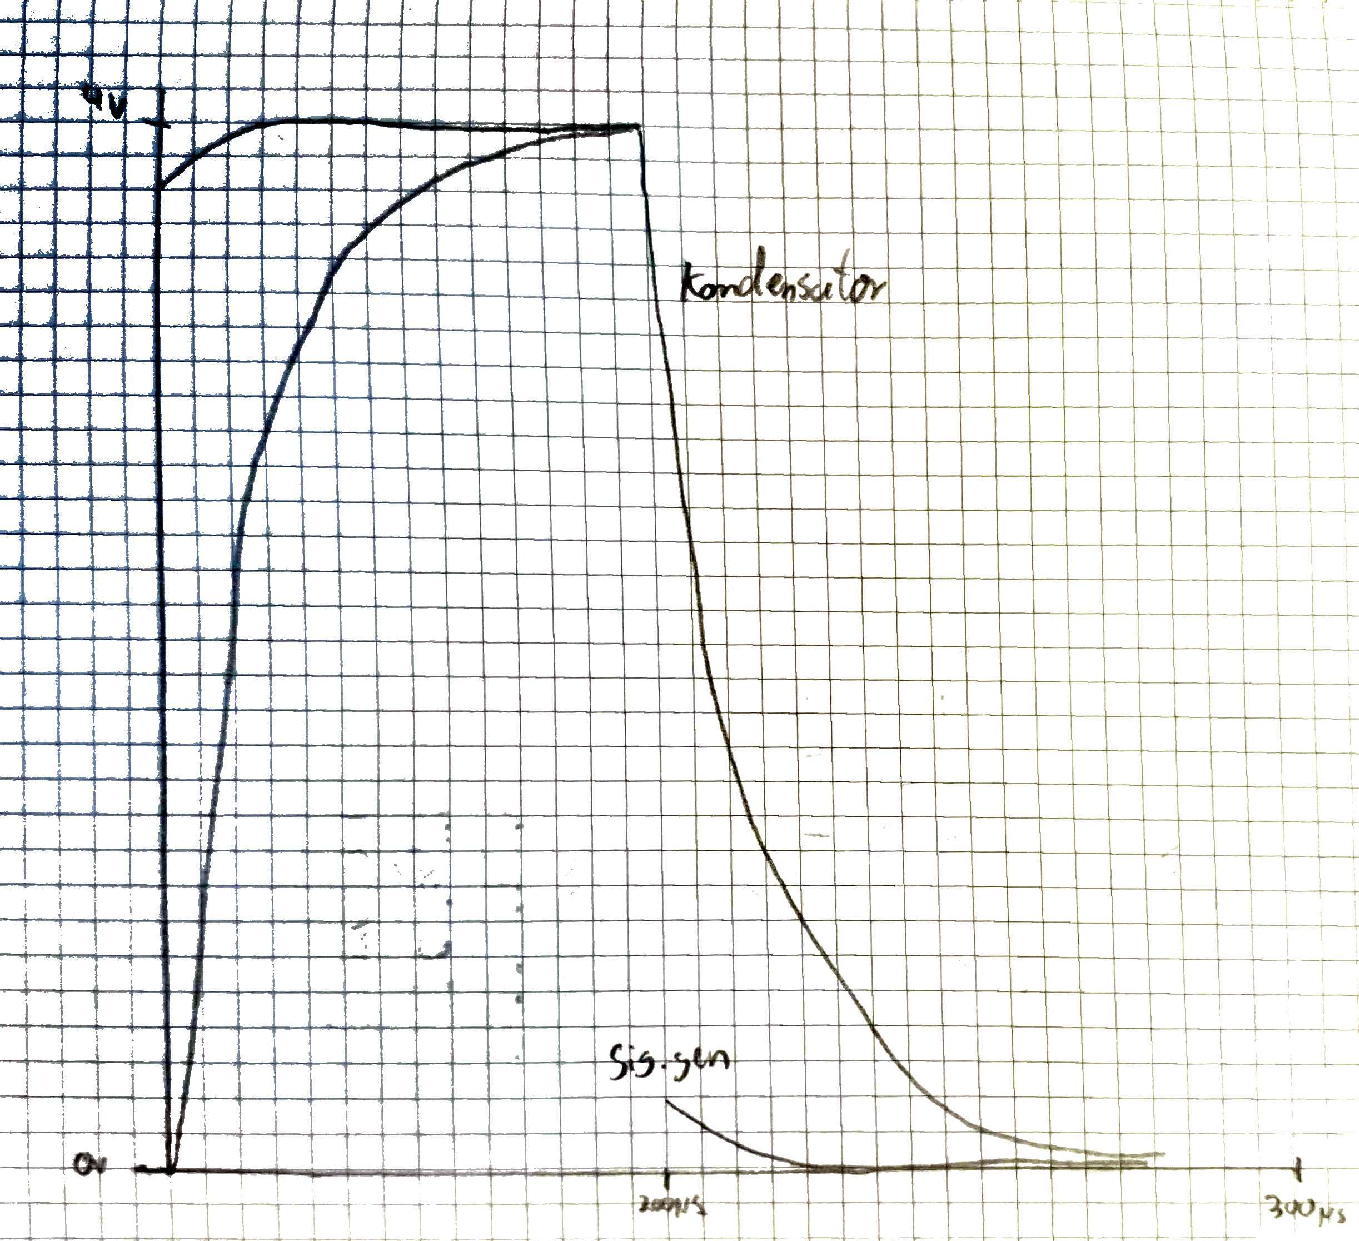
\includegraphics[height=6cm]{figurer/RC-figur.pdf}
    \caption{Spenningen over kondensatoren og signalgeneratoren}
    \label{fig:rc-resultater}
\end{figure}

$\tau$ ble målt til å være $17\cdot 10^{-6}s$

\subsection{CMOS logikk}

Figur~\ref{fig:cmos-resultater} viser spenningene målt ved punktene D og Q fra CMOS logikk kretsen som vist i Figur~\ref{fig:rc}. Målingene av D og Q er gjort i Volt.

\begin{figure}[!htb]
    \centering
    \begin{tabular}{|c|c|c|c|c|}
        \hline
        \textbf{A} & \textbf{B} & \textbf{C} & \textbf{D} & \textbf{Q} \\ \hline
        0 & 0 & 0 & 9 & 8.4 \\
        1 & 0 & 0 & 9 & 0 \\
        1 & 1 & 0 & 9 & 0 \\
        1 & 0 & 1 & 9 & 0 \\
        1 & 1 & 1 & 0 & 0 \\
        0 & 0 & 1 & 9 & 8.4 \\
        0 & 1 & 0 & 9 & 8.4 \\
        0 & 1 & 1 & 0 & 8.7 \\ \hline
    \end{tabular}
    \caption{Målingene av CMOS spenningene}
    \label{fig:cmos-resultater}
\end{figure}